\chapter{RESULTADOS E DISCUSSÃO}
\label{cap:04}
Para o desenvolvimento foi utilizado duas maquinas virtuais com o sistema Operacional \textit {OpenSuse}, com o software de transmissão de arquivos atráves do protocolo torrent, qBittorrent, instalado.
Para realizar um acesso remoto à essas máquinas, foi utilizado o cliente de conexão  \textit{\ac{ssh}} Putty e nele configurado a opção de controle SSH X11 \textit {forwarding}, para que a a interface gráfica da máquina virtual fosse aberta pela maquina host.

Foi utilizado o mesmo arquivo .torrent em ambas as máquinas e os testes não foram feito de forma simultaneas para que não houvesse distribuição de banda e elas pudessem ter o máximo desempenho nos testes, dessa forma é possível analisar as transparências de concorrência e replicação. 

Na primeira máquina virtual foi realizado o download do arquivo conectando com todos as \ac{seed} disponíveis. Quando conectado a 10 \ac{seed}, foi obtido uma disponibilidade do arquivo de 10.046, e uma velocidade média de download de 8.2MiB/S, conforme a figura \ref{fig:disponibilidade 10 seeds}  
\begin{figure}[!htb]
\centering
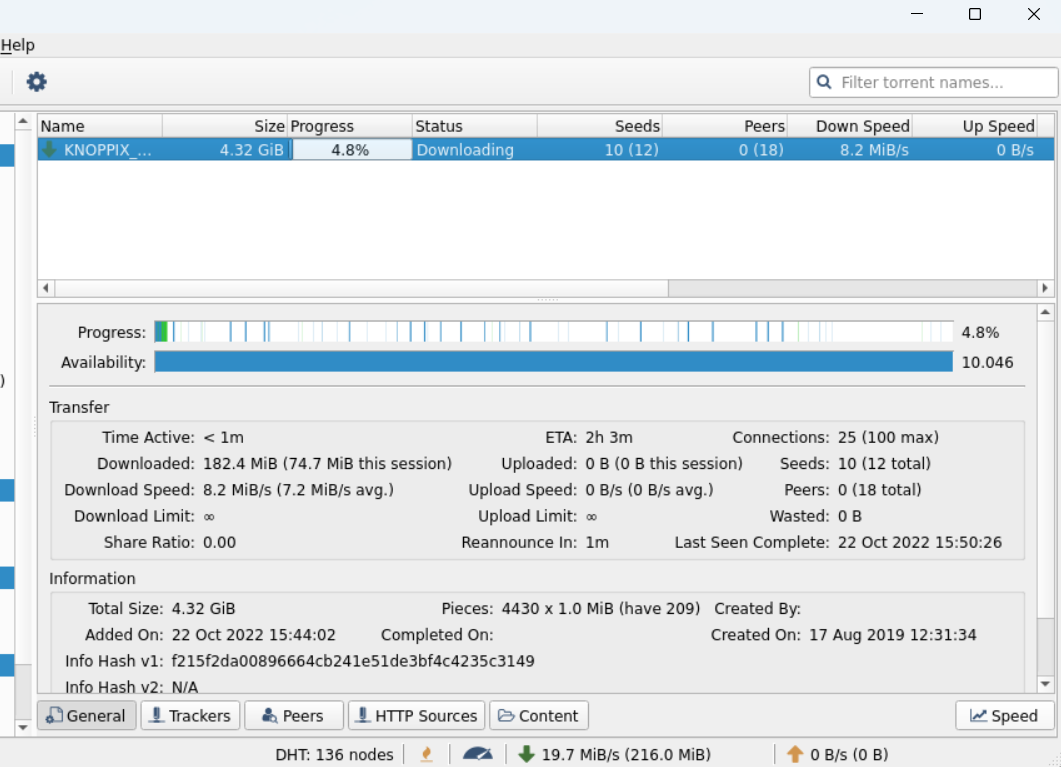
\includegraphics[width=0.6\textwidth]{./images/disponibilidade 10 seeds.png}
\caption{Disponibilidade do arquivo com 10 seeds}
\label{fig:disponibilidade 10 seeds}
\end{figure}

Na segunda máquina virtual foi limitado a quantidade de peers conectados com o intuito de diminuir a concorrência e o desempenho, Quando conectado a 5 \ac{seed}, foi obtido uma disponibilidade de 5.256, e uma velocidade média de donwload de 1.6MiB/S, conforme a figura \ref{fig:disponibilidade_5_seeds}
\begin{figure}[!htb]
\centering
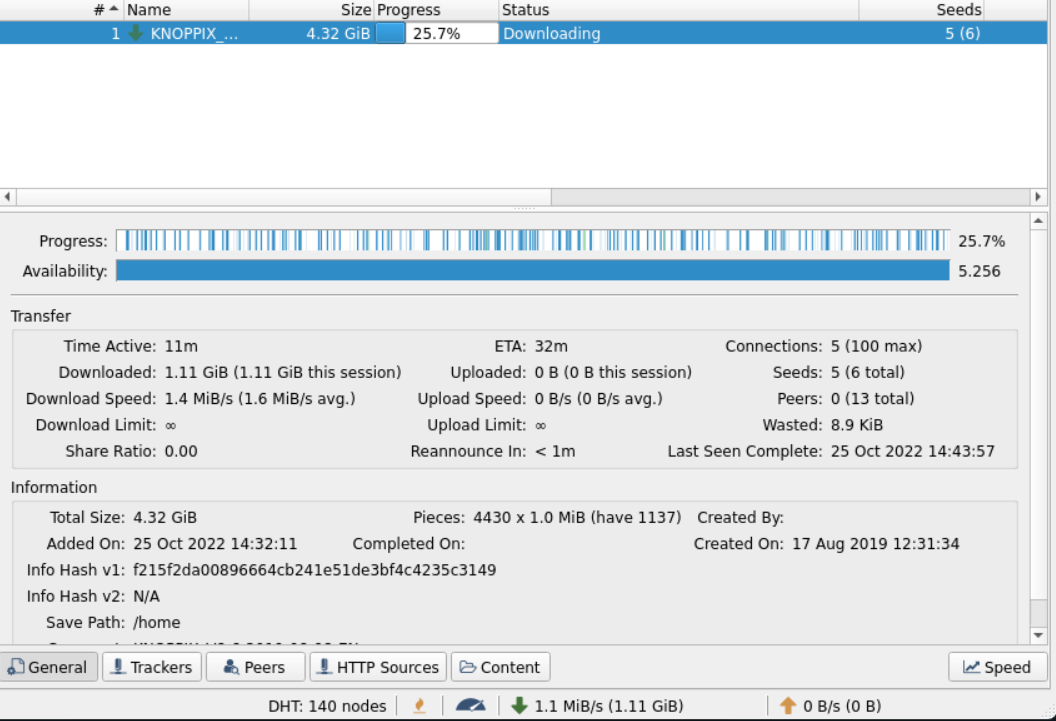
\includegraphics[width=0.65\textwidth]{./images/disponibilidade 5 seeds.png} 
\caption{Disponibilidade do arquivo com 5 seeds}
\label{fig:disponibilidade_5_seeds}
\end{figure}

Foi realizado um teste sobre a disponibilidade e velocidade de transmissão do arquivo .torrent, quando conectado a somente um seed, mostrando um gráfico de velocidade de download estabilizado com velocidade de 832.1KiB/S após a mudança para somente 1 seed conforme a figura \ref{fig:velocidade_1_seed}.
\begin{figure}[!htb]
\centering
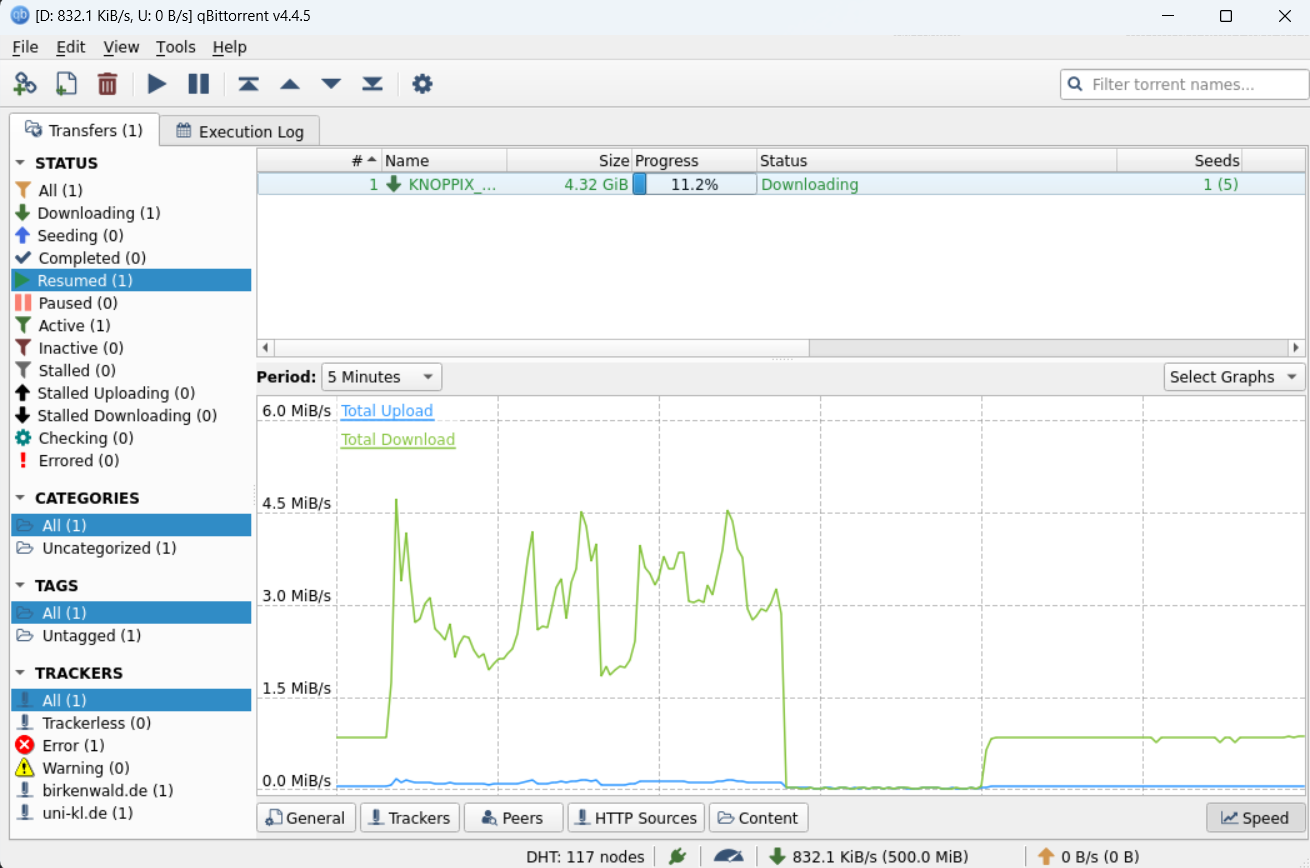
\includegraphics[width=0.7\textwidth]{./images/velocidade download 1 seed.png}
\caption{Velocidade de Download com 1 seed}
\label{fig:velocidade_1_seed}
\end{figure}